Fig.~\ref{fig:TE} compares the execution time and the power consumption of 
\texttt{covariance} program variants with and without a good tiling size
configuration ($32\times16\times1$).
We can see from comparing the pink/purple line with the green line that 
proper tile size reduces execution time by up to $4\times$ (always 
at least $2\times$ performance increase) and results in
minimum execution time.  

We can also see from the smooth execution time line that 
with tiling there are 3 performance breaks and without tilting 1 performance break.
The fastest executions of variants without tiling all have maxfuse set -- approx $45\%$ improvement
of performance.
In the case of program variants with tiling, 
\begin{enumerate}
\item 1st break. Turning vectorization OFF had ~$45\%$ improvement 
\item 2nd break. Setting maxfuse on had ~$10\%$  improvement
\item 3rd break. Set maxfuse on \textbf{and} turn vectorization ON had ~$100\%$ improvement
\end{enumerate}
%    overall 18 sec to 2+ sec better than 6x
\textbf{It is interesting to note how one optimization (i.e. maxfuse) can impact the functionality
   of a second optimization (i.e. vectorization) so drastically. The increase of
loop size and scope that maxfuse produces allows vectorization to go from a severe lost to a major win 
(thus turning vectorization on with maxfuse leads to minimum execution time). }

Optimizations can greatly change the power required by an application. 
E.g. maxfuse takes the tiled version from 108W to 150W (~40\% increase), the untiled
from 120W to 170W (again about 40\% increase). Also note that turning vectorization 
off increased power by a couple of Watts.
For this application the power increases are more than made up by the execution
time reductions -- least energy is the quickest execution time.

\textbf{Hypothesis: maxfuse allows more memory references to be simultaneously
visible to the compiler and vectorization increase greatly -- as does overlap
of memory and ALU increasing power used considerably.}

%Questions:  1 Is assumption true?
%        2 How does a machine learning function make sure that it does
%           not give up on vectorization until everything is viable?
%        3 Are there relationships between optimizations that can be
%           applied across applications?
%        4 Can this be generalized? more apps more optimizations?

%Issue we may want to bring up with John: My knee-jerk reaction when I see
%
%this type of graph is to start thinking about how to improve optimizations
%internal to the compiler. Should I be driving more to improved optimization
%
%ordering criteria or use this information  on how to better initialize
%the machine learning algorithms to increase convergence. (which I don't
%really understand.)

\begin{figure}[bt]
    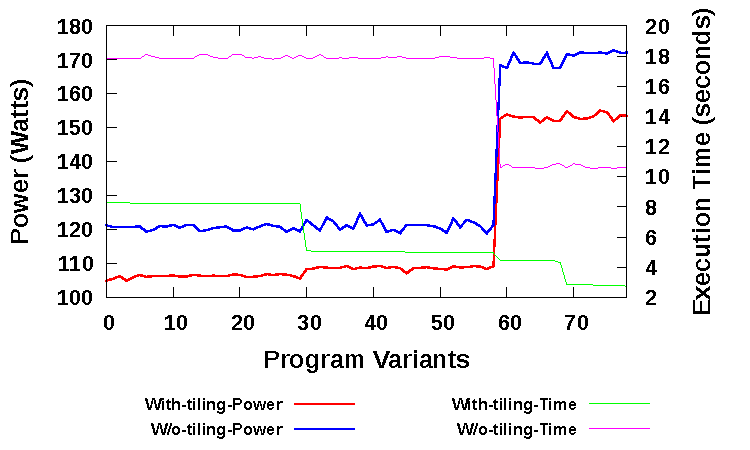
\includegraphics[width=3.5in]{Covariance}
%    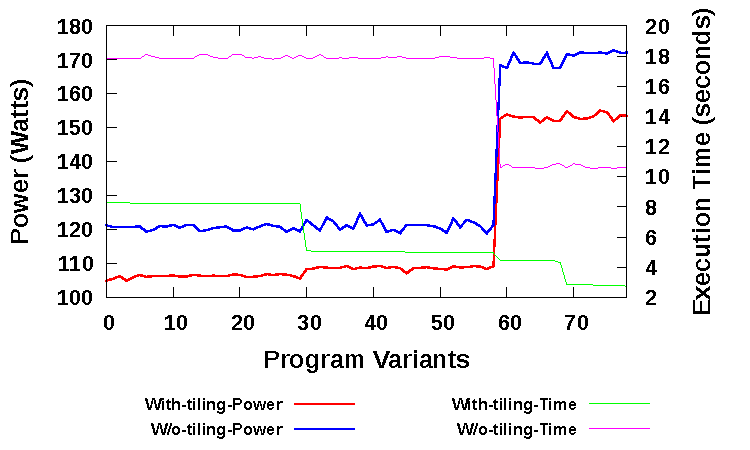
\includegraphics{Covariance}
    \caption{Graph showing the execution time and the power of \texttt{covariance} Polybench program variants with 
and without loop tiling on SandyBridge Processor (sorted by execution time of program variants with loop tiling turned on).
 The jumps of power are caused by ``maxfuse'' loop transformation. The three breaks of the execution time line (with loop tiling)
are caused by turning vectorization off, turning maxfuse on, and turning both maxfuse and vectorization on, respectively.}
    \label{fig:TE}
\end{figure}
